\chapter{Ajuste da imagem}

O InVesalius não garante a correta ordem das imagens pois depende de informações que estão presentes nas imagens, algumas vezes essas imagens tem as informações incorretas ou não seguem o padrão DICOM. Dessa forma é recomendável confirmar se a lesão ou algum outro marco anatômico presente em um determinado paciente é exibido no lado correto da imagem. Caso não seja, é possível utilizar as ferramentas de espelhar a imagem ou inverter eixos. Também para o alinhamento da imagem, existe a ferramenta de rotação da imagem.

\section{Espelhar}

É possível espelhar um dos lados da imagem de modo que eles se invertam, para isso é necessário ir no menu, \textbf{Ferramentas}, \textbf{Imagem}, \textbf{Espelhar} e clicar em uma das seguintes opções (figura~\ref{fig:menu_img_mirroring_axis_pt}):

\begin{itemize}
	\item Direita - Esquerda
	\item Anterior - Posterior
	\item Superior - Inferior
\end{itemize}

\begin{figure}[!htb]
\centering
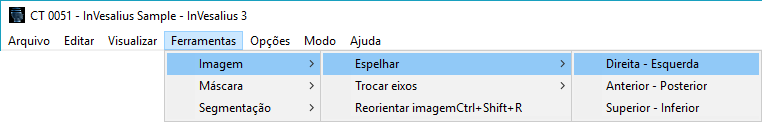
\includegraphics[scale=0.4]{menu_img_mirroring_axis_pt.png}
\caption{Menu para ativar espelhar um dos lados da imagem.}
\label{fig:menu_img_mirroring_axis_pt}
\end{figure}



\section{Inverter Eixo}

\section{Rotacionar} 